
% Plantilla para un Trabajo Fin de Grado de la Universidad de Granada,
% adaptada para el Doble Grado en Ingeniería Informática y Matemáticas.
%
%  Autor: Mario Román.
%  Licencia: GNU GPLv2.
%
% Esta plantilla es una adaptación al castellano de la plantilla
% classicthesis de André Miede, que puede obtenerse en:
%  https://ctan.org/tex-archive/macros/latex/contrib/classicthesis?lang=en
% La plantilla original se licencia en GNU GPLv2.
%
% Esta plantilla usa símbolos de la Universidad de Granada sujetos a la normativa
% de identidad visual corporativa, que puede encontrarse en:
% http://secretariageneral.ugr.es/pages/ivc/normativa
%
% La compilación se realiza con las siguientes instrucciones:
%   pdflatex --shell-escape main.tex
%   bibtex main
%   pdflatex --shell-escape main.tex
%   pdflatex --shell-escape main.tex

% Opciones del tipo de documento
\documentclass[oneside,openright,titlepage,numbers=noenddot,openany,headinclude,footinclude=true,
  cleardoublepage=empty,abstractoff,BCOR=5mm,paper=a4,fontsize=12pt]{scrreprt}

% Paquetes de latex que se cargan al inicio. Cubren la entrada de
% texto, gráficos, código fuente y símbolos.
\usepackage[utf8]{inputenc}
\usepackage[T1]{fontenc}
\usepackage{fixltx2e}
\usepackage{graphicx} % Inclusión de imágenes.
\usepackage{grffile}  % Distintos formatos para imágenes.
\usepackage{longtable} % Tablas multipágina.
\usepackage{wrapfig} % Coloca texto alrededor de una figura.
\usepackage{rotating}
\usepackage[normalem]{ulem}
\usepackage{amsmath}
\usepackage{textcomp}
\usepackage{amssymb}
\usepackage{capt-of}
\usepackage[colorlinks=true]{hyperref}
\usepackage{tikz} % Diagramas conmutativos.
\usepackage{minted} % Código fuente.
\usepackage{natbib}
\usepackage{bm}
\usepackage{todonotes}
\usetikzlibrary{positioning}
% Plantilla classicthesis
\usepackage[beramono,eulerchapternumbers,linedheaders,parts,a5paper,dottedtoc,
manychapters,pdfspacing]{classicthesis}

% Geometría y espaciado de párrafos.
\setcounter{secnumdepth}{0}
\usepackage{enumitem}
\setitemize{noitemsep,topsep=0pt,parsep=0pt,partopsep=0pt}
\setlist[enumerate]{topsep=0pt,itemsep=-1ex,partopsep=1ex,parsep=1ex}
\usepackage[top=1in, bottom=1.5in, left=1in, right=1in]{geometry}
\setlength\itemsep{0em}
\setlength{\parindent}{0pt}
\usepackage{parskip}

% Profundidad de la tabla de contenidos.
\setcounter{secnumdepth}{3}

% Usa el paquete minted para mostrar trozos de código.
% Pueden seleccionarse el lenguaje apropiado y el estilo del código.
\usepackage{minted}
\usemintedstyle{colorful}
\setminted{fontsize=\small}
\renewcommand{\theFancyVerbLine}{\sffamily\textcolor[rgb]{0.5,0.5,1.0}{\oldstylenums{\arabic{FancyVerbLine}}}}

% Archivos de configuración.
%------------------------
% Bibliotecas para matemáticas de latex
%------------------------
\usepackage{amsthm}
\usepackage{amsmath}
\usepackage{tikz}
\usepackage{tikz-cd}
\usetikzlibrary{shapes,fit}
\usepackage{bussproofs}
\EnableBpAbbreviations{}
\usepackage{mathtools}
\usepackage{scalerel}
\usepackage{stmaryrd}

%------------------------
% Estilos para los teoremas
%------------------------
\theoremstyle{plain}
\newtheorem{theorem}{Theorem}
\newtheorem{proposition}{Proposition}
\newtheorem{lemma}{Lemma}
\newtheorem{corollary}{Corollary}
\theoremstyle{definition}
\newtheorem{definition}{Definition}
\newtheorem{proofs}{Proof}
\theoremstyle{remark}
\newtheorem{remark}{Remark}
\newtheorem{exampleth}{Example}

\begingroup\makeatletter\@for\theoremstyle:=definition,remark,plain\do{\expandafter\g@addto@macro\csname th@\theoremstyle\endcsname{\addtolength\thm@preskip\parskip}}\endgroup

%------------------------
% Macros
% ------------------------

% Aquí pueden añadirse abreviaturas para comandos de latex
% frequentemente usados.
\newcommand*\diff{\mathop{}\!\mathrm{d}}
\newcommand{\R}{\mathbb{R}}
% \newcommand{\E}{\mathbb{E}}
\newcommand{\bmu}{\bm{\mu}}
\newcommand{\bx}{\bm{x}}
\newcommand{\bX}{\bm{X}}
\newcommand{\bz}{\bm{z}}
\newcommand{\bZ}{\bm{Z}}
\newcommand{\bv}{\bm{v}}
\newcommand{\bh}{\bm{h}}
\newcommand{\bSigma}{\bm{\Sigma}}
\newcommand{\bpi}{\bm{\pi}}
\newcommand{\bLambda}{\bm{\Lambda}}
\newcommand{\btheta}{\bm{\theta}}
\newcommand{\bnu}{\bm{\nu}}
\newcommand{\bV}{\bm{V}}


\newcommand{\V}{\mathcal{V}}
\newcommand{\D}{\mathcal{D}}
\newcommand{\X}{\mathcal{X}}
\newcommand{\I}{\mathcal{I}}

\newcommand\ddfrac[2]{\frac{\displaystyle #1}{\displaystyle #2}}

\newcommand\E[2]{\mathbb{E}_{#1}\Big[#2\Big]}
\newcommand\KL[2]{KL\Big(#1 \bigm| #2\Big)}
\newcommand{\bigCI}{\mathrel{\text{\scalebox{1.07}{$\perp\mkern-10mu\perp$}}}}
\newcommand{\bigCD}{\centernot{\bigCI}}

\DeclareMathOperator*{\argmax}{arg\,max}
\DeclareMathOperator*{\argmin}{arg\,min}
  % En macros.tex se almacenan las opciones y comandos para escribir matemáticas.
\input{classicthesis-config} % En classicthesis-config.tex se almacenan las opciones propias de la plantilla.

% Color institucional UGR
% \definecolor{ugrColor}{HTML}{ed1c3e} % Versión clara.
\definecolor{ugrColor}{HTML}{c6474b}  % Usado en el título.
\definecolor{ugrColor2}{HTML}{c6474b} % Usado en las secciones.

% Datos de portada
\usepackage{titling} % Facilita los datos de la portada
\author{Luis Antonio Ortega Andrés}
\date{\today}
\title{Statistical Models with Variational Methods}

% Portada
\usepackage{datetime}
\renewcommand\maketitle{
  \begin{titlepage}
    \begin{addmargin}[-2.5cm]{-3cm}
      \begin{center}
        \large  
        \hfill
        \vfill

        \begingroup
        \color{ugrColor}\spacedallcaps{\thetitle} \\ \bigskip
        \endgroup

        \spacedlowsmallcaps{\theauthor}

        \vfill

        Bachelor's Thesis \\ \medskip
        Computer Science and Mathematics \\  \bigskip\bigskip


        \textbf{Tutor}\\
        Serafín Moral Callejón \\ \bigskip

        \spacedlowsmallcaps{Faculty of Science} \\
        \spacedlowsmallcaps{H.T.S. of Computer Engineer and Telecommunications} \\ \medskip
        
        \textit{Granada, \today}

        \vfill                      

      \end{center}  
    \end{addmargin}       
  \end{titlepage}}

\usepackage{wallpaper}

\begin{document}

\maketitle
\tableofcontents

\chapter*{Abstract}

Some introduction about how important Variational methods are nowadays and what this project is about.

\ctparttext{
  \color{black}
  \begin{center}
    Chapter description
  \end{center}
}
\part{Basic Concepts}

\chapter{Probability}

All our theory will be made under the assumption that there is a \emph{referential
set} \(\Omega\), set of all possible outcomes of an experiment. Any subset of
\(\Omega\) will be called \emph{event}.

\begin{definition}
Let \(\mathcal{P}(\Omega)\) be the power set of \(\Omega\). Then, \(\mathcal{F} \subset \mathcal{P}(\Omega)\) is called a
\emph{\(\sigma\)-algebra} if it satisfies:
\begin{itemize}
\item \(\Omega \in \mathcal{F}\).
\item \(\mathcal{F}\) is closed under complementation.
\item \(\mathcal{F}\) is closed under countable unions.
\end{itemize}
From these properties it follows that \(\emptyset \in \mathcal{F}\) and that \(\mathcal{F}\)
is closed under countable intersections.

The tuple \((\Omega, \mathcal{F})\) is called a \emph{measurable space}.
\end{definition}

\begin{definition}
A \emph{probability} \(P\) over \((\Omega, \mathcal{F})\) is a mapping
\(P: \mathcal{F} \to [0,1]\) which satisfies
\begin{itemize}
\item \(P(\alpha) \geq 0 \ \ \forall \alpha \in \mathcal{F}\).
\item \(P(\Omega) = 1\).
\item \(P\) is countably additive, that is, if \(\{\alpha_i\}_{i \in \mathbb{N}}
  \subset \mathcal{F}\), is a countable collection of pairwise disjoint sets,
  then
  \[
  P\big(\bigcup_{i\in \mathbb{N}}\alpha_i\big) = \sum_{i\in \mathbb{N}}P(\alpha_i).
  \]
\item For any sequence {\(\{\alpha_n\}_{n \in \mathbb{N}}\)} such that \(\alpha_i \subset
  \alpha_{i+1} \ \forall i \in \mathbb{N}\) and \(\alpha_n
  \xrightarrow{n \to \infty} \Omega\), then
  \[P(\alpha_n)
  \xrightarrow{n \to \infty} P(\Omega) = 1.\]
\end{itemize}
\end{definition}

The first condition guarantees non negativity. The second one states that the
\emph{trivial event} has the maximal possible probability of 1. The third condition implies that given two mutually disjoint events,
the probability of either one of them occurring is equal to the sum of the
probabilities of each one. The last condition sets an upper semi-continuity.

From these conditions it follows that \(P(\emptyset) = 0\) and \(P(\alpha \cup \beta)
= P(\alpha) + P(\beta) - P(\alpha \cap \beta)\).

The triple \((\Omega, \mathcal{F}, P)\) is called a \emph{probability space}.

\begin{definition}
A function \(f:\Omega_1 \to \Omega_2\) between two
measurable spaces is said to be \emph{measurable} if \(f^{-1}(\alpha) \in \mathcal{F}_1\) for every \(\alpha \in \mathcal{F}_2\).
\end{definition}

\begin{definition}
A \emph{random variable} is a measurable function \(X:\Omega \to E\) from a probability
space \((\Omega, \mathcal{F}, P)\) to a measurable space \(E\).

The probability of \(X\) taking a value on a measurable set \(S \subset E\) is
written as
\[
P(X \in S) = P(\{a \in \Omega \ | \ X(a) \in S \}).
\]
\end{definition}

We will adopt the following notation from now on: random variables will be
denoted with an upper case letter like \(X\) and a set of variables with a
bold symbol like \(\bm{X}\) The meaning of \(P(state)\) will be clear without a reference to the variable.
Otherwise \(P(X = state)\) will be used.
We will denote by \(P(x)\) the probability of \(X\) taking a specific value.

Also \(P(x \text{ or } y) = P(x \cup y)\) and \(P(x,y) = P(x \cap y)\).

We will define some concepts regarding a joint distribution \(P(x,y)\), that is
to say, the probability of both random variables \(x\) and \(y\).

\begin{definition}
The \emph{cumulative distribution function} of a random variable \(X\) is the
function given by:
\[
F_X (x) = P(X \leq x)
\]
where the right-hand side represents the probability of the random variable
taking value below of equal to \(x\).
\end{definition}

\begin{definition}
When the image of a random variable \(X\) is countable, the random variable is called
\emph{discrete random variable}, its \emph{probability mass function} \(p\) gives the
probability of it being equal to some value.
\[
p(x) = P(X = x)
\]
If the image is uncountable then \(X\) is called a \emph{continuous random
  variable} and its \emph{probability density function} \(f\) is a non-negative
Lebesgue-integrable such that
\[
F_X(x) = P(X \leq x) = \int_{-\infty}^x f(u) du
\]
\end{definition}

\begin{definition}
A \emph{marginal distribution} \(P(x)\) of the joint distribution is the
distribution of a single variable given by
\[
P(x) = \sum_y P(x,y) \hspace{2cm} P(x) = \int_y P(x,y)
\]
\end{definition}

We can understand this as the probability of an event irrespective of the outcome
of the other variable.

\begin{definition}
The \emph{conditional probability} of \(X\) given \(Y\) is defined as

\[
p(x|y) = \frac{p(x,y)}{p(y)}
\]

If \(p(y) = 0\) then it is not defined.
\end{definition}

With this definition the
conditional probability is the probability of one event occurring in the presence of a
second event. \\

\begin{theorem}
  \textbf{(Bayes' theorem)}. Given two random variables \(X,Y\), then
  \[
  P(x|y)= \frac{P(y|x)P(x)}{P(y)}
  \]
\end{theorem}



\begin{exampleth}
Consider a study where the relation of a disease \(d\) and an habit \(h\)
is being investigated. Suppose that \(p(d)=10^{-5}\), \(p(h)=0.5\) and \(p(h|d) = 0.9\). What is the
probability that a person with habit \(h\) will have the disease \(d\)?

\[
p(d|h) = \frac{p(d,h)}{p(h)} = \frac{p(h|d)p(d)}{p(h)} =
\frac{ 0.9 \times 10^{-5}}{ 0.5 } = 1.8 \times 10^{-5}
\]

If we set the probability of having habit \(h\) to a much lower value as \(p(h) =
0.001\), then the above calculation gives approximately \(1/100\). Intuitively, a smaller number of people have the habit and most of them have the
desease. This means that the relation between having the desease and the habit
is stronger now compared with the case where more people had the habit.
\end{exampleth}

Now suppose we have some observed data \(\mathcal{D}\) and we want to learn about
a set of parameters \(\theta\). Using Bayes' rule we got that

\[
p(\theta|\mathcal{D}) = \frac{p(\mathcal{D}|\theta)p(\theta)}{p(\mathcal{D})} =
\frac{p(\mathcal{D}|\theta)p(\theta)}{ \int_{\theta} p(\mathcal{D}|\theta)p(\theta)}
\]

This shows how from a \emph{generative model} \(p(\mathcal{D}|\theta)\) of the dataset
and a \emph{prior} belief \(p(\theta)\), we can infer the \emph{posterior} distribution
\(p(\theta|\mathcal{D})\). \\

\begin{definition}
We say that two random variables \(X\) and \(Y\) are \emph{independent} if knowing one of them doesn't give any extra information about the other. Mathematically,
\[
p(x,y) = p(x) p(y)
\]
From this it follows that if \(X\) and \(Y\) are independent, then \(p(x|y) = p(x)\).
\end{definition}

\begin{definition}
\todo[inline]{TODO: conditional independence}
\end{definition}

%%%%%%%%%%%%%%%%%%%%%%%%%%%%%%%%%%%%%%%%%%%%%%%%%%%%%%%%%%%%%%%%%%%%%%%%%%%%%%%%
%%%%%%%%%%%%%%%%%%%%%%%%%%%%%%%%%%%%%%%%%%%%%%%%%%%%%%%%%%%%%%%%%%%%%%%%%%%%%%%%
%%%%%%%%%%%%%%%%%%%%%%%%%%%%%%% Graphical Models %%%%%%%%%%%%%%%%%%%%%%%%%%%%%%%
%%%%%%%%%%%%%%%%%%%%%%%%%%%%%%%%%%%%%%%%%%%%%%%%%%%%%%%%%%%%%%%%%%%%%%%%%%%%%%%%
%%%%%%%%%%%%%%%%%%%%%%%%%%%%%%%%%%%%%%%%%%%%%%%%%%%%%%%%%%%%%%%%%%%%%%%%%%%%%%%%

\chapter{Graphical models}

\begin{definition}
A \emph{graph} \(G = (V,E)\) is a set of vertices or nodes \(V\) and edges \(E\subset
V\times V\) between them.
If \(V\) is a set of ordered pairs then the graph is called a \emph{directed
  graph}, otherwise if \(V\) is a set of unordered pairs it is called an \emph{undirected graph}.
\end{definition}

\begin{figure*}[h]
\centering
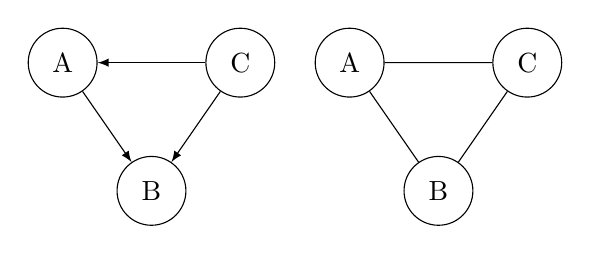
\begin{tikzpicture}[
  node distance=1cm and 0.5cm,
  mynode/.style={draw,circle,text width=0.5cm,align=center}
]

\node[mynode] (a) {A};
\node[mynode,below right=of a] (b) {B};
\node[mynode,above right=of b] (c) {C};

\node[mynode, right=of c] (d) {A};
\node[mynode,below right=of d] (e) {B};
\node[mynode,above right=of e] (f) {C};

\path (c) edge[-latex] (a)
(a) edge[-latex] (b)
(b) edge[latex-] (c);

\draw (d) -- (e) -- (f) -- (d);

\end{tikzpicture}
\caption{Example of directed and undirected graph, respectively.}
\label{fig:graphs}
\end{figure*}

\begin{definition}
In a directed graph \(G = (V, E)\), a \emph{directed path} \(A \to B\) is a sequence of vertices \({A = A_0,
  A_1,\dots,A_{n-1}, A_n = B}\) where \((A_i, A_{i-1}) \in E \ \forall i \in
0,\dots ,n\).

If \(G\) is a undirected graph, \(A \to B\) is an \emph{undirected path} if \(\forall i \in
0,\dots, n, \ (A_i, A_{i-1}) \in E\) or  \((A_{i-1}, A_{i}) \in E\)
\end{definition}

\begin{definition}
Let \(A,B\) be two vertices of a directed graph \(G\). If \(A \to B\) is a
directed path and \(B \not \to A\) (meaning there isn't a directed path from
\(B\) to \(A\)), then \(A\) is called an \emph{ancestor} of \(B\) and \(B\) is called a \emph{descendant} of \(A\).
\end{definition}

For example, in the figure \ref{fig:graphs}, \(C\) is an ancestor of \(B\).

\begin{definition}
A \emph{directed acyclic graph (DAG)} is a directed graph such that no directed path between any two nodes revisits a vertex.
\end{definition}


\begin{figure}[h]
\centering
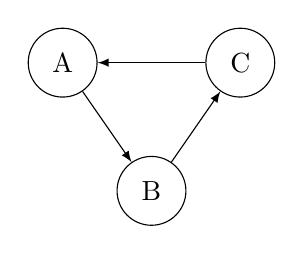
\begin{tikzpicture}[
  node distance=1cm and 0.5cm,
  mynode/.style={draw,circle,text width=0.5cm,align=center}
]

\node[mynode] (a) {A};
\node[mynode,below right=of a] (b) {B};
\node[mynode,above right=of b] (c) {C};

\path (c) edge[-latex] (a)
(a) edge[-latex] (b)
(b) edge[-latex] (c);

\end{tikzpicture}
\captionof{figure}{Example of graph which isn't a DAG.}
\label{fig:not_dag}
\end{figure}

As we can see in the figure \ref{fig:not_dag}, \(A \to B \to C \to A \to B\) is a
path from \(A\) to \(B\) that revisits \(A\).

Now where are going to define some relations between nodes in a DAG.

\begin{definition}
The \emph{parents} of a node \(A\) is the set of nodes \(B\) such that there is a
directed edge from \(B\) to \(A\). The same applies for the \emph{children} of a node.

The \emph{Markov blanket} of a node is composed by the node itself, its children, its parents and the parents
of its children.
\end{definition}


\begin{figure}[h]
\centering
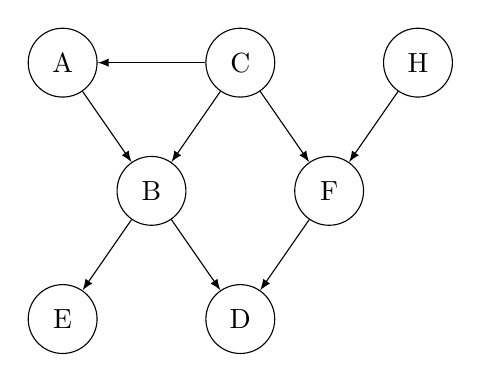
\begin{tikzpicture}[
  node distance=1cm and 0.5cm,
  mynode/.style={draw,circle,text width=0.5cm,align=center}
]

\node[mynode] (a) {A};
\node[mynode,below right=of a] (b) {B};
\node[mynode,above right=of b] (c) {C};
\node[mynode,below right=of b] (d) {D};
\node[mynode,below left=of b] (e) {E};
\node[mynode,above right=of d] (f) {F};
\node[mynode, above right=of f] (h) {H};

\path (c) edge[-latex] (a)
(a) edge[-latex] (b)
(b) edge[latex-] (c)
(b) edge[-latex] (e)
(c) edge[-latex] (f)
(b) edge[-latex] (d)
(f) edge[-latex] (d)
(h) edge[-latex] (f)
;

\end{tikzpicture}
\captionof{figure}{Directed acyclic graph}
\label{fig:relations}
\end{figure}

\begin{definition}
In a graph, the \emph{neighbors} of a node are those directly connected
to it.
\end{definition}

We can use figure \ref{fig:relations} to reflect on these definitions. The parents
of \(B\) are \(pa(B) = \{A,C\}\) and its children are \(ch(B) = \{E,D\}\). Taking this into account, its neighbors
are \(ne(B) = \{A,C,E,D\}\) and its Markov blanket is \(\{A,B,C,D,E,F\}\).

\begin{definition}
A \emph{graphical model} is a probabilistic model for which a graph expresses the
conditional dependence structure between random variables.
\end{definition}

Commonly, they provide a graph-based representation for encoding a multi-dimensional
distribution representing a set of independences that hold in the specific
distribution. The most commonly used are \emph{Bayesian networks} and \emph{Markov random
fields}, which differ in the set of independences they can encode and the
factorization of the distribution that they include.

\section{Belief networks}

Consider we have \(N\) variables with the corresponding distribution
\(p(x_1,\dots,x_N)\). Let \(\mathcal{E}\) be a set of indexes such as \texttt{evidence}
\(=\{x_e = \times _e \ | \ e \in \mathcal{E}\}\). Inference could be made by brute
force:

\[
p(x_i = \times _i \ | \ \texttt{evidence}) = \frac{ \int_{ j \not \in
\mathcal{E}, j \neq i } p(\texttt{evidence}, x_j, x_i = \times_i)}{ \int_{ j
\not \in \mathcal{E} } p(\texttt{evidence}, x_j)}
\]

The notation when using discrete variables is analogous replacing integration
with summations.

Lets suppose all these variables are binary, this calculation will require
\(O(2^{N-\#\mathcal{E}})\) operations. Also, all entries of a table \(p(x_1,\dots,
x_N)\) take \(O(2^N)\) space.

This is unpractical when taking into account millions of variables. The
underlying idea of belief networks is to specify which variables are independent
of others, factoring the joint probability distribution.

\begin{definition}
A \emph{belief network} is a distribution of the form
\[
p(x_1,\dots,x_N) = \prod_{i=1}^{N}p(x_i | pa(x_i))
\]
\end{definition}

We can write it as a DAG where the \(i^{th}\) node corresponds to the factor
\(p(x_i|pa(x_i))\).


\clearpage
Cites so the references appear (testing) \cite{koller_friedman,barber,wainwright}
\bibliographystyle{plain}
\bibliography{refs}
\end{document}
